\documentclass[conference]{IEEEtran}
\IEEEoverridecommandlockouts
\usepackage{cite}
\usepackage{amsmath,amssymb}
\usepackage{graphicx}
\usepackage{booktabs}
\usepackage{multirow}
\usepackage{xcolor}
\usepackage{tikz}
\usetikzlibrary{positioning,arrows.meta,fit,backgrounds,calc,shapes.geometric}
\usepackage{pgfplots}
\pgfplotsset{compat=1.17}
\usepackage[hidelinks]{hyperref}
\usepackage{url}
\usepackage{array}

\definecolor{kblue}{HTML}{2F5BD3}
\definecolor{kgold}{HTML}{C9A24A}
\definecolor{kred}{HTML}{B91C1C}
\definecolor{kamber}{HTML}{D97706}
\definecolor{kgreen}{HTML}{15803D}
\definecolor{kgray}{HTML}{475569}
\definecolor{kmid}{HTML}{0F172A}

\def\UrlBreaks{\do\/\do-\do\_\do\.}
\begin{document}

\title{KAVACH: An On-Device, Multilingual Scam-Call Shield for Indian Phone Users with Llama~3.2~1B on Arm CPUs%
\thanks{This paper is the Phase~1 technical submission of team KAVACH to the \textbf{Arm Bharat AI-SoC Challenge 2026--27}, Problem Statement~3: \emph{Cybersecurity and Digital Safety}. Source code, models, benchmarks and the full technical report: \url{https://github.com/siddhaantxsingh/KAVACH}.}}

\author{
\IEEEauthorblockN{Siddhant Singh, Bogavalli Sai Akhilash, Shivansh Bose}
\IEEEauthorblockA{\textit{Manipal Institute of Technology}\\
\textit{Manipal Academy of Higher Education}\\
Manipal, Karnataka, India}
\and
\IEEEauthorblockN{Dr. Rahul Ratnakumar}
\IEEEauthorblockA{\textit{Faculty Mentor}\\
\textit{Manipal Institute of Technology}\\
\textit{Manipal Academy of Higher Education}\\
Manipal, Karnataka, India}
}

\maketitle

\begin{figure*}[!t]
\centering
\resizebox{\textwidth}{!}{%
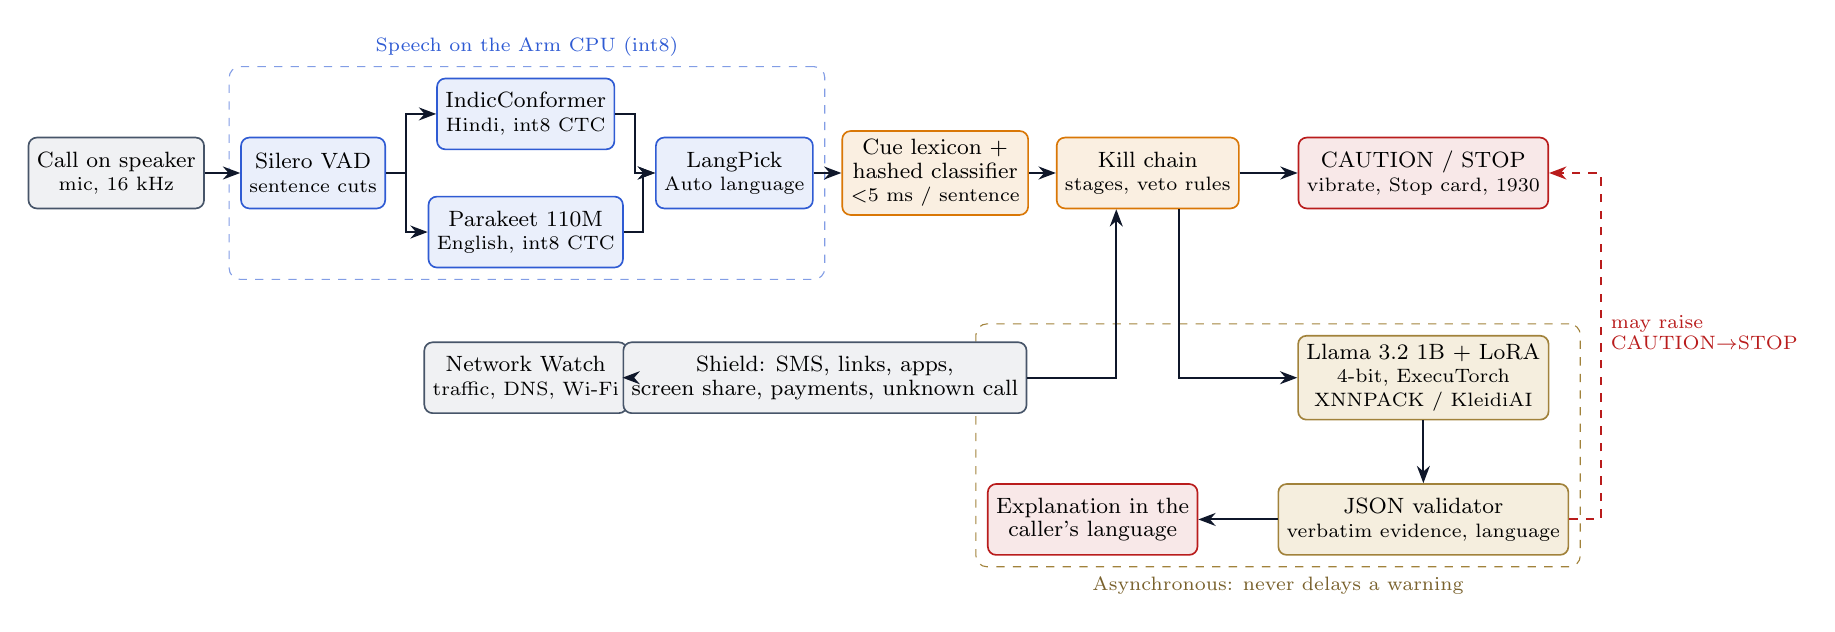
\begin{tikzpicture}[
  font=\footnotesize, >={Stealth[length=2.2mm]},
  box/.style={draw, rounded corners=3pt, align=center, minimum height=9mm, inner sep=3pt, line width=0.6pt},
  sp/.style={box, fill=kblue!10, draw=kblue},
  det/.style={box, fill=kamber!12, draw=kamber},
  ll/.style={box, fill=kgold!18, draw=kgold!80!black},
  ob/.style={box, fill=kred!10, draw=kred},
  src/.style={box, fill=kgray!8, draw=kgray},
  ar/.style={->, line width=0.7pt, draw=kmid}
]
\node[src] (mic) at (0,0) {Call on speaker\\[-1pt]\scriptsize mic, 16 kHz};
\node[sp]  (vad) at (2.5,0) {Silero VAD\\[-1pt]\scriptsize sentence cuts};
\node[sp]  (hi)  at (5.2,0.75) {IndicConformer\\[-1pt]\scriptsize Hindi, int8 CTC};
\node[sp]  (en)  at (5.2,-0.75) {Parakeet 110M\\[-1pt]\scriptsize English, int8 CTC};
\node[sp]  (lp)  at (7.85,0) {LangPick\\[-1pt]\scriptsize Auto language};
\node[det] (cue) at (10.4,0) {Cue lexicon +\\[-1pt]hashed classifier\\[-1pt]\scriptsize $<$5 ms / sentence};
\node[det] (kc)  at (13.1,0) {Kill chain\\[-1pt]\scriptsize stages, veto rules};
\node[ob]  (alert) at (16.6,0) {CAUTION / STOP\\[-1pt]\scriptsize vibrate, Stop card, 1930};
\node[src] (nw)  at (5.2,-2.6) {Network Watch\\[-1pt]\scriptsize traffic, DNS, Wi-Fi};
\node[src] (shield) at (9.0,-2.6) {Shield: SMS, links, apps,\\[-1pt]screen share, payments, unknown call};
\node[ll]  (llama) at (16.6,-2.6) {Llama 3.2 1B + LoRA\\[-1pt]\scriptsize 4-bit, ExecuTorch\\[-1pt]\scriptsize XNNPACK / KleidiAI};
\node[ll]  (val) at (16.6,-4.4) {JSON validator\\[-1pt]\scriptsize verbatim evidence, language};
\node[ob]  (exp) at (12.4,-4.4) {Explanation in the\\[-1pt]caller's language};
\draw[ar] (mic) -- (vad);
\draw[ar] (vad.east) -- ++(2.5mm,0) |- (hi.west);
\draw[ar] (vad.east) -- ++(2.5mm,0) |- (en.west);
\draw[ar] (hi.east) -- ++(2.5mm,0) |- (lp.west);
\draw[ar] (en.east) -- ++(2.5mm,0) |- (lp.west);
\draw[ar] (lp) -- (cue);
\draw[ar] (cue) -- (kc);
\draw[ar] (kc) -- (alert);
\draw[ar] (nw) -- (shield);
\draw[ar] (shield.east) -| ([xshift=-4mm]kc.south);
\draw[ar] ([xshift=4mm]kc.south) |- (llama.west);
\draw[ar] (llama) -- (val);
\draw[ar] (val) -- (exp);
\draw[ar, dashed, draw=kred] (val.east) -- ++(4mm,0) |- node[pos=0.27, right, align=left, text=kred]{\scriptsize may raise\\[-2pt]\scriptsize CAUTION$\to$STOP} (alert.east);
\begin{scope}[on background layer]
\node[draw=kblue!60, dashed, rounded corners, fit=(vad)(hi)(en)(lp), inner sep=4pt, label={[text=kblue]above:\scriptsize Speech on the Arm CPU (int8)}] {};
\node[draw=kgold!80!black, dashed, rounded corners, fit=(llama)(val)(exp), inner sep=4pt, label={[text=kgold!60!black]below:\scriptsize Asynchronous: never delays a warning}] {};
\end{scope}
\end{tikzpicture}}
\caption{KAVACH pipeline on one Android phone. Blue: speech front-end; amber: always-on detector; gold: Llama advisor; red: what the user sees. No component uses the network.}
\label{fig:arch}
\end{figure*}

\begin{abstract}
Phone fraud in India increasingly happens on a \emph{live call}: a caller poses as police, a bank or a courier, isolates the victim and steers a payment while the call is still running. Cloud-based detectors cannot hear such calls without sending private audio off the phone. This paper presents \textbf{KAVACH}, a single Android application that listens to a call the user has put on speaker, recognises Hindi, Hinglish and English speech on the phone, and warns the user \emph{during} the call, with no internet permission at all. Speech is cut into sentences by a voice-activity detector and recognised by two int8 CTC models (AI4Bharat IndicConformer for Hindi, NVIDIA Parakeet~110M for English); an \emph{Auto} mode runs both on every sentence and keeps the transcript whose words are real words of its language. A sub-5\,ms detector (cue lexicon, hashed linear classifier and a multi-channel kill chain) raises CAUTION or STOP, and a LoRA-fine-tuned Llama~3.2~1B, quantised to 4~bits and run with ExecuTorch on the Arm CPU, explains the alert in the caller's language. On a mid-range Snapdragon~7s~Gen~2 phone, both speech models together run about $5\times$ faster than real time, a one-minute listening run drew 385\,mA for the whole phone without heating, and Llama decodes 11.5--11.9 tokens/s. In three real cellular calls from an unknown number, a Hindi ``digital arrest'' scam and an English KYC scam reached STOP during the call and a genuine bank call raised no warning. On 1,000 unseen synthetic calls the detector reached STOP on 93.4\,\% of scams with no genuine call stopped. An ablation shows that cross-channel fusion adds STOPs at the risky action (an app install or remote access during the call) but no earlier warnings, and can blame a genuine call for an unrelated scam SMS. Fine-tuning raised Llama's valid-verdict rate from 71\,\% to 100\,\% and scam accuracy from 38\,\% to 89\,\% (full-precision model, synthetic data).
\end{abstract}

\begin{IEEEkeywords}
Scam detection, on-device AI, speech recognition, Llama, ExecuTorch, Arm, LoRA, Android, privacy, Hindi
\end{IEEEkeywords}

\section{Introduction}

Indian phone scams have shifted from single messages to orchestrated conversations. In a typical ``digital arrest'' call the fraudster claims to be from a cyber-crime branch, says a parcel booked on the victim's Aadhaar contains drugs, forbids the victim to tell anyone, and finally asks for a transfer to an ``RBI safe account''. Every step is spoken; nothing is written. The scale is large: the Ministry of Home Affairs told Parliament that Indians lost about Rs.~22,845 crore to cyber fraud in 2024, about 206\,\% more than in 2023~\cite{mha_loss}, and digital-arrest incidents on the National Cyber Crime Reporting Portal rose from 39,925 in 2022 to 1,23,672 in 2024, with reported losses growing from about Rs.~91 crore to Rs.~1,935 crore~\cite{mha_da}.

A protection that only reads SMS or URLs arrives after the money has gone, a bank-side check sees only the payment, and a protection that uploads call audio to a server creates a new privacy risk of its own and fails where the network is weak. KAVACH (Sanskrit for \emph{armour}) takes the opposite route: everything runs on the user's phone. The design goals were
(i)~\emph{on-device only}: the main app does not even request Android's \texttt{INTERNET} permission and never stores audio;
(ii)~\emph{Indian languages}: Hindi, Hinglish and English, including callers who switch mid-call;
(iii)~\emph{early and calm}: warn before the payment step, with zero false STOPs on genuine calls as a hard target;
(iv)~\emph{explainable}: say in plain words, in the caller's language, what trick is being played and what to do (call 1930, the national cyber-crime helpline);
(v)~\emph{Arm-efficient}: run in real time on a mid-range phone CPU with measured speed, memory, battery and heat.

\textbf{Contributions.}
\begin{itemize}
\item A one-phone architecture that listens to a speaker-phone call through Android's accessibility audio exception, with automatic start on calls from unknown numbers and a self-check that detects when Android silently stops the permission (Section~\ref{sec:arch}).
\item A bilingual sentence-level speech front-end with per-sentence language choice (\emph{Auto}, 92.7\,\% correct), raising Hindi telephone-band detection from 0\,\% to 58\,\% STOP on 100 unseen calls (Sections~\ref{sec:speech}, \ref{sec:hindi}).
\item A fast, explainable detector (16-category cue lexicon, hashed classifier, multi-channel kill chain) that is ported bit-exactly from Python to Kotlin (336 parity checks) and stopped no genuine call in any evaluated set (Sections~\ref{sec:det}, \ref{sec:calllevel}).
\item A LoRA-tuned Llama~3.2~1B advisor, exported to a 4-bit ExecuTorch file, with a strict JSON contract and a validator that removes invented evidence; fine-tuning raises scam accuracy from 38\,\% to 89\,\% (Sections~\ref{sec:llama}, \ref{sec:llamaeval}).
\item Measurements on a real Snapdragon~7s~Gen~2 phone and three real cellular calls, two negative results that changed the design, and all code, data generators and results released (Section~\ref{sec:eval}).
\end{itemize}

The rest of the paper is organised as follows. Section~\ref{sec:related} reviews related work, Section~\ref{sec:problem} defines the threat model, Section~\ref{sec:arch} describes the system, Section~\ref{sec:impl} the data and implementation, Section~\ref{sec:eval} the evaluation, Section~\ref{sec:disc} lessons and limitations, and Section~\ref{sec:concl} concludes.

\section{Related Work}\label{sec:related}

\subsection{Protection against phone fraud}
Deployed protections fall into four broad categories (Table~\ref{tab:approaches}). Number-reputation services label known spam numbers but cannot see what is said and are defeated by fresh or spoofed numbers. SMS and link filters see only text that arrives on the phone. Cloud call screening can hear the conversation, but the audio leaves the phone. Bank-side transaction monitoring acts only when the payment is made, after the victim has already been persuaded. KAVACH sits in the gap: it hears the conversation itself, during the call, on the phone.

\begin{table}[t]
\caption{Categories of scam protection (qualitative)}
\label{tab:approaches}
\centering
\footnotesize
\setlength{\tabcolsep}{3pt}
\begin{tabular}{@{}lccc@{}}
\toprule
Approach & Hears the call & Offline & Hindi explanation \\
\midrule
Number reputation & no & partly & no \\
SMS / link filters & no & often & rarely \\
Cloud call screening & yes, audio leaves & no & varies \\
Bank transaction checks & no, after payment & no & no \\
\textbf{KAVACH} & \textbf{yes, on device} & \textbf{yes} & \textbf{yes} \\
\bottomrule
\end{tabular}
\end{table}

\subsection{On-device speech recognition}
Conformer~\cite{conformer} encoders combine self-attention with convolution and dominate modern recognisers; Fast Conformer~\cite{fastconformer} reduces the cost of attention so long audio can be processed cheaply. Connectionist temporal classification (CTC)~\cite{ctc} lets the network emit symbols frame by frame and is decoded greedily, which is far cheaper than beam search on a phone. AI4Bharat's IndicConformer, trained on large Indian-language corpora such as IndicVoices~\cite{indicvoices}, covers Hindi including English loanwords, and NVIDIA's Parakeet~\cite{parakeet} provides compact English models. sherpa-onnx~\cite{sherpa} runs int8 ONNX exports of both on Arm CPUs, together with the Silero voice-activity detector~\cite{silero}.

\subsection{Small language models on Arm}
Large language models such as Llama~3~\cite{llama3} can explain fraud patterns in natural language, but a phone needs a small, quantised model. Groupwise 4-bit weight quantisation and rotation-based methods such as SpinQuant~\cite{spinquant} make Llama~3.2~1B fit in under 1\,GB. ExecuTorch~\cite{executorch} exports PyTorch models to a portable \texttt{.pte} program whose XNNPACK backend uses Arm KleidiAI micro-kernels~\cite{kleidiai} for 4-bit matrix multiplication on Arm CPUs. Low-rank adaptation (LoRA)~\cite{lora} specialises such a model by training two small matrices per layer, which can be merged into the base weights before export so that run-time cost is unchanged.

\subsection{Lightweight classification and attack chains}
Feature hashing~\cite{hashing} maps words and character fragments into a fixed number of buckets, giving fixed-size, vocabulary-free linear models that are trivial to port between languages. The kill-chain idea from intrusion analysis~\cite{killchain} treats an attack as a sequence of stages: a single indicator is weak evidence, a sequence of stages is strong. KAVACH applies it across channels: what is said on a call, which message and link arrive, which app is opened and how the network behaves.

\section{Problem and Threat Model}\label{sec:problem}

We model a scam call as a progression through five stages: \emph{contact} (an unknown number claims to be police, CBI, a bank, a courier, TRAI or a utility), \emph{hook} (an authority claim combined with an identity hook or threat), \emph{isolation} (``don't disconnect, don't tell anyone''), \emph{action} (share an OTP, open a link, install a remote-access app, share the screen) and \emph{payment} (transfer, UPI collect request, ``safe account''). The goal is to reach STOP before the payment stage while never raising STOP on a genuine call. Table~\ref{tab:types} lists the twelve scam types in KAVACH's playbook, paraphrased from I4C, RBI and bank advisories.

\begin{table}[t]
\caption{Scam types in the KAVACH playbook}
\label{tab:types}
\centering
\footnotesize
\setlength{\tabcolsep}{3pt}
\begin{tabular}{@{}ll@{}}
\toprule
Identifier & Scam \\
\midrule
\texttt{digital\_arrest} & fake police / CBI, ``digital arrest'' \\
\texttt{courier\_parcel} & parcel with illegal items \\
\texttt{kyc\_bank} & fake KYC / account block \\
\texttt{upi\_collect\_refund} & UPI collect request / fake refund \\
\texttt{investment\_trading} & investment / trading group \\
\texttt{job\_task} & part-time job / task scam \\
\texttt{family\_emergency} & ``your son is in trouble'' \\
\texttt{electricity\_bill} & electricity disconnection \\
\texttt{sim\_telecom} & TRAI / SIM disconnection \\
\texttt{lottery\_prize} & lottery / prize / KBC \\
\texttt{remote\_support} & fake customer care, remote access \\
\texttt{loan\_app} & instant loan app, harassment \\
\bottomrule
\end{tabular}
\end{table}

\textbf{Adversary.} The scammer controls what is said, can switch language, can avoid obvious trigger words, can send links, APKs and SMS during the call, and can try to calm the victim with small talk. The scammer cannot run code on the victim's phone before the victim installs something. \textbf{Assumptions.} The user has installed KAVACH, granted its permissions and puts unknown calls on speaker (KAVACH's optional dialer does this automatically). \textbf{Out of scope.} Calls the user never puts on speaker, and compromised phones.

\section{System Architecture}\label{sec:arch}

\begin{figure*}[!t]
\centering
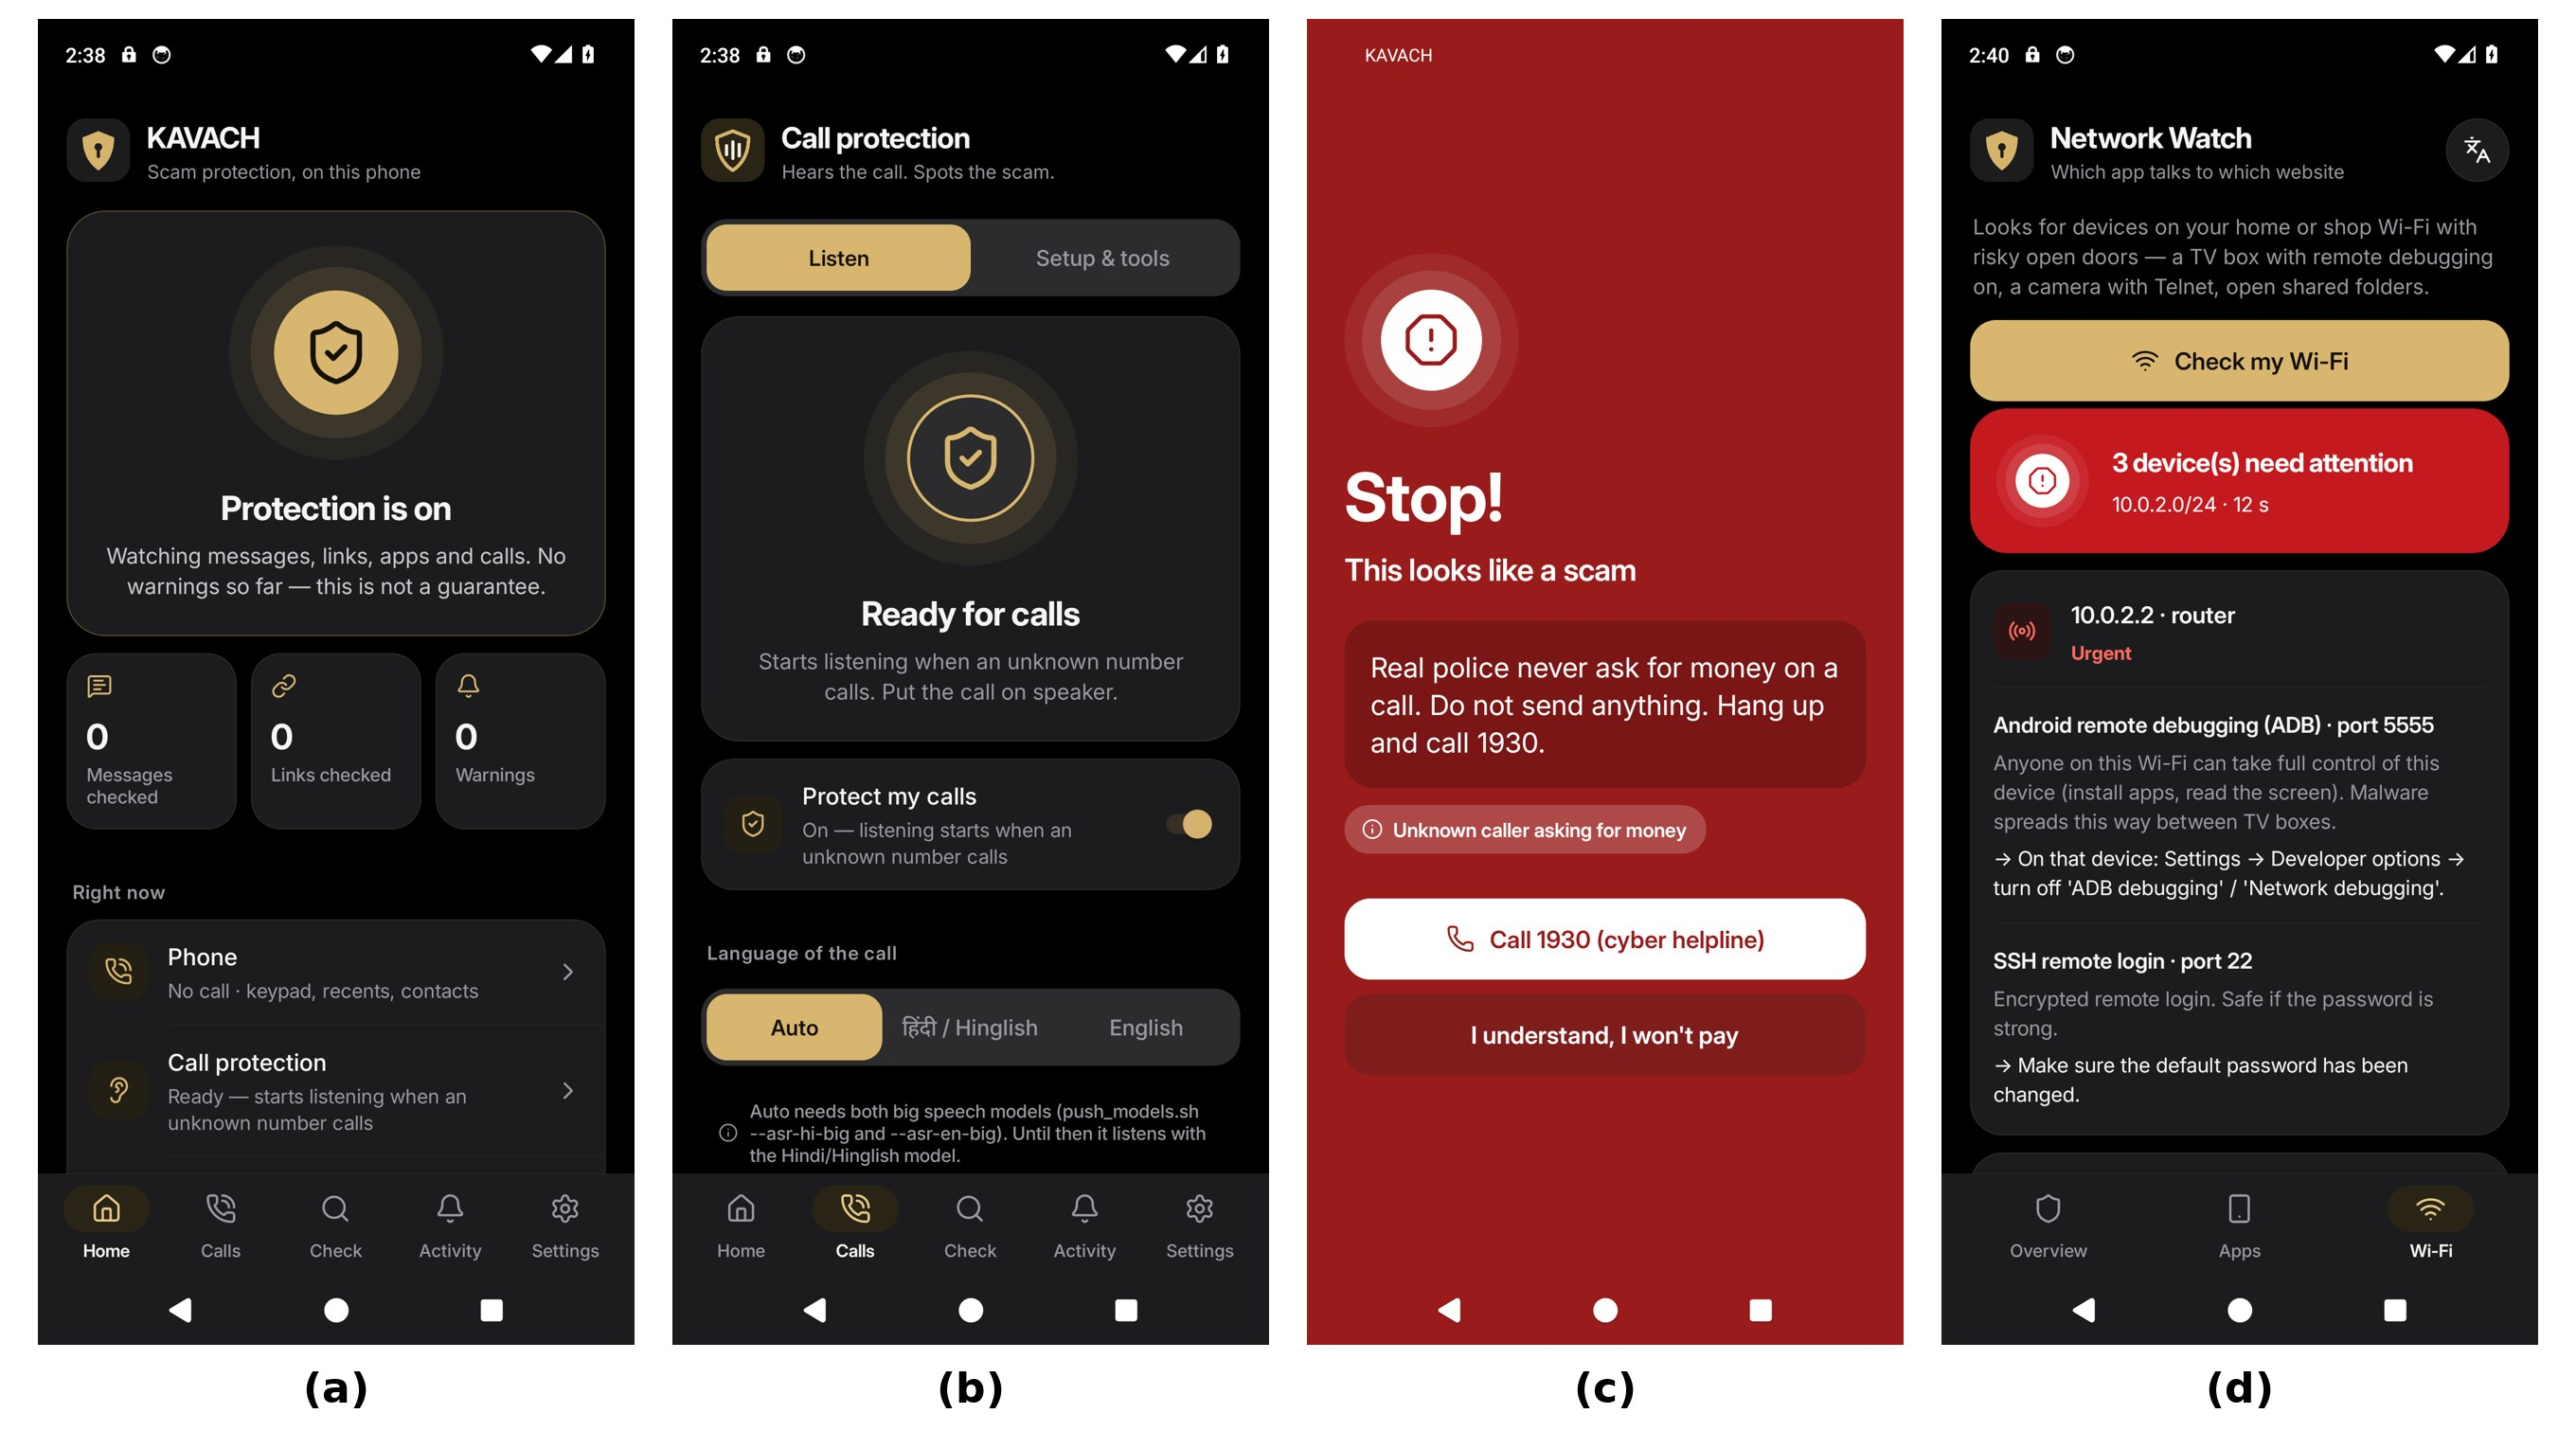
\includegraphics[width=0.86\textwidth]{fig/app_ui.jpg}
\caption{The app. (a)~Home with live protection status and on-phone counters. (b)~Call protection, Auto language. (c)~Stop card raised by a scam SMS and link. (d)~Network Watch finding risky devices on the home Wi-Fi.}
\label{fig:ui}
\end{figure*}

Fig.~\ref{fig:arch} shows the pipeline. Three on-device sources feed one kill chain: \emph{call listening} (what is said), \emph{Shield} (messages, links, apps, screen sharing, payment apps, and the fact that an unknown number is calling) and the optional \emph{Network Watch} app (per-app traffic, website look-ups and risky devices on the home Wi-Fi). Llama is invoked only when the level rises, on its own thread, so the always-on path never waits for it. Fig.~\ref{fig:ui} shows the main screens.

\subsection{One-phone call listening}
During a cellular call Android gives the microphone to the call and feeds every other app's recording with silence. The documented exception is an enabled accessibility service~\cite{androidaudio}. KAVACH declares a minimal service that reads no screen content and performs no actions; while it runs, the app keeps hearing a call the user has put on speaker. A phone-state listener and a contacts look-up start listening automatically when an \emph{unknown} number calls. Warnings during a call are silent (vibration and a full-screen card): a spoken warning would be sent into the call and would also mute KAVACH's own capture.

During our tests Android stopped the app once (after the default dialer changed) and marked the service as crashed while its switch still showed ``on''; every call recording was then silenced. The app now compares the enabled setting with the services Android actually runs (\texttt{getEnabledAccessibilityServiceList}) and checks \texttt{isClientSilenced()} on its own recording during a call, telling the user how to fix it instead of failing silently.

\subsection{Speech front-end and Auto language}\label{sec:speech}
Audio is captured at 16\,kHz mono in 100\,ms chunks with automatic gain control and noise suppression off; it lives only in a memory buffer for one sentence. Silero VAD cuts audio into sentences (0.5\,s minimum silence, 12\,s maximum). Each sentence is recognised whole by an int8 CTC model, with a partial result every 2\,s while the caller speaks (Table~\ref{tab:frontend}). A placement check estimates the signal-to-noise ratio from 20\,ms frame powers and tells the user to move the phone closer if needed, and an own-voice filter ignores sentences heard while KAVACH itself speaks.

\begin{table}[t]
\caption{Speech front-end}
\label{tab:frontend}
\centering
\footnotesize
\setlength{\tabcolsep}{3pt}
\begin{tabular}{@{}lll@{}}
\toprule
Stage & Model / method & Size \\
\midrule
VAD & Silero VAD, 512-sample windows & 0.6 MB \\
Hindi / Hinglish & IndicConformer, 120M, int8 CTC & 198 MB \\
English & Parakeet TDT-CTC 110M, int8 & 126 MB \\
Fallback & streaming Zipformer (hi / en) & 69 / 188 MB \\
Language & LangPick (word lists) & $<$1 MB \\
\bottomrule
\end{tabular}
\end{table}

In \emph{Auto} mode both models recognise every sentence. Each model turns speech of the other language into words that are not real words of its own language (the English model writes Hindi as nonsense syllables, and vice versa), so LangPick keeps the transcript whose words are more often real, common words of its language:
\begin{equation}
s = (k_{en} - k_{hi}) + W\,(c_{en} - c_{hi}),
\end{equation}
where $k$ is the share of words among the 20,000 most frequent words of that language (wordfreq~\cite{wordfreq}), $c$ the share among the 200 most frequent (mostly function words), both counted over $n{+}1$ words so that a one-word fragment cannot win, and $W{=}1$. English is chosen if $s>0.2$; a sentence whose score lies within 0.15 of that margin keeps the previous sentence's language, and warnings follow the majority of the last three sentences. Hinglish naturally goes to the Hindi model, which writes English loanwords that the lexicon also knows in Devanagari.

\subsection{Always-on detector}\label{sec:det}
The detector runs after every sentence and at least every 3\,s. It has three layers.

\textbf{Cue lexicon.} 698 phrases in 16 categories (Table~\ref{tab:cues}), each in English, romanised Hinglish and Devanagari, plus 208 mixed-script loanword variants mined from what the Hindi model actually writes. Phrase rules allow gaps of up to four words, and a request is ignored when a nearby word negates it, so ``never share your OTP'' counts as safety advice. Three \emph{victim-side} categories catch the person next to the phone reading out an OTP, saying they are paying, or pleading not to be arrested.

\begin{table}[t]
\caption{Cue categories of the lexicon}
\label{tab:cues}
\centering
\footnotesize
\setlength{\tabcolsep}{3pt}
\begin{tabular}{@{}ll@{}}
\toprule
Category & Example \\
\midrule
authority\_police / \_bank & ``CBI'', ``RBI officer'' \\
identity\_misuse & ``your Aadhaar is linked'' \\
threat / urgency & ``arrest warrant'', ``within two hours'' \\
isolation & ``don't tell anyone'' \\
credential\_request & ``tell me the OTP'' \\
remote\_access / link\_click & ``install AnyDesk'', ``open the link'' \\
payment\_request & ``transfer to safe account'' \\
reward\_greed / family\_emerg. & ``you have won'', ``your son'' \\
safety\_advice & ``never share your OTP'' \\
victim\_sharing / \_paying / \_fear & ``main transfer kar raha hoon'' \\
\bottomrule
\end{tabular}
\end{table}

\textbf{Hashed classifier.} A logistic regression~\cite{hashing} scores the last 120 tokens using FNV-1a hashes of words, word pairs and 3--5 letter fragments, plus cue categories and category pairs (about 1\,MB). Every score decomposes into per-word contributions, which become the evidence words shown to the user. The same design scores SMS and URLs.

\textbf{Kill chain.} Evidence from all channels fades with a channel-specific half-life (10\,min for calls, 30\,min for messages and links, 24\,h for apps). The level is sticky within a session, so small talk cannot calm it. Table~\ref{tab:rules} lists the rules. The classifier adds CAUTION or STOP when it stays above 0.8 for two ticks, and can veto a weak rule-only STOP while it is confidently benign ($<0.5$); strong rules are never vetoed. Thresholds were tuned on development sets only.

\begin{table}[t]
\caption{Kill-chain rules}
\label{tab:rules}
\centering
\footnotesize
\setlength{\tabcolsep}{3pt}
\begin{tabular}{@{}ll@{}}
\toprule
Rule & Level \\
\midrule
isolation + authority & STOP (vetoable) \\
authority + identity misuse + threat & STOP \\
two different action / payment requests & STOP \\
hook + action, no safety advice heard & STOP \\
victim complying + scam pretext & STOP \\
suspicious call + risky action, same call & STOP \\
unknown call + dangerous link / APK / screen share & STOP \\
evidence from two channels & STOP \\
weighted score $\geq 7$ / $\geq 3$ & STOP / CAUTION \\
payment app in unknown call $>$3 min & CAUTION \\
\bottomrule
\end{tabular}
\end{table}

\subsection{Llama advisor}\label{sec:llama}
On CAUTION or STOP, the transcript window, active cues and the three most relevant playbook entries are given to Llama~3.2~1B~\cite{llama3}. The constant system prefix (rules, schema, scam types; 1,361 characters) is pre-filled into the KV cache when the app starts and re-armed after every alert, which halves the time to the first token. Decoding is greedy and stops as soon as the JSON object closes. Each generation is limited to 35\,s, set from the phone measurements (warm path $\approx$15\,s, cold path of the fine-tuned file $\approx$26\,s); the timer covers waiting for a background prefix prefill, the prompt prefill and the generation, not model loading. The model must return one JSON object (Table~\ref{tab:json}).

\begin{table}[t]
\caption{Llama output contract}
\label{tab:json}
\centering
\footnotesize
\setlength{\tabcolsep}{3pt}
\begin{tabular}{@{}lp{0.68\columnwidth}@{}}
\toprule
Field & Allowed values \\
\midrule
\texttt{scam} & true / false \\
\texttt{type} & one of Table~\ref{tab:types}, or none \\
\texttt{stage} & none, contact, hook, isolation, action, payment \\
\texttt{confidence} & 0.0--1.0 (clamped) \\
\texttt{evidence} & $\leq$3 quotes, verbatim from the transcript \\
\texttt{say} & $\leq$35 words, in the call's language \\
\texttt{action} & none, continue\_with\_care, verify\_independently, do\_not\_share, do\_not\_pay, hang\_up \\
\bottomrule
\end{tabular}
\end{table}

\textbf{Validator.} Enumerations are enforced (\texttt{"scam": "maybe"} fails, a bug found by our unit tests), evidence not found verbatim in the transcript is dropped and the confidence capped, advice that copies the prompt's example or is in the wrong language is replaced by vetted playbook text and labelled as such, and an unfinished last sentence is cut. On invalid output the model is asked once more. Llama can raise CAUTION to STOP (confidence $\geq 0.8$, stage $\geq$ isolation) but can never lower a rule STOP, which also limits the damage of any prompt injection spoken by the caller.

\textbf{Fine-tuning and export.} We generated 4,000 training and 400 development instruction pairs with the same prompt code the phone runs and trained LoRA~\cite{lora} adapters (Table~\ref{tab:lora}). The merged model was exported with ExecuTorch~1.4 using 8-bit dynamic activations and 4-bit groupwise weights ($g{=}32$) plus 4-bit embeddings, giving an 820\,MB file (Meta's SpinQuant file is 1,083\,MB).

\begin{table}[t]
\caption{LoRA configuration}
\label{tab:lora}
\centering
\footnotesize
\setlength{\tabcolsep}{3pt}
\begin{tabular}{@{}ll@{}}
\toprule
Setting & Value \\
\midrule
Base & Llama-3.2-1B-Instruct \\
Rank / alpha / dropout & 16 / 32 / 0.05 \\
Target layers & q, k, v, o, gate, up, down \\
Batch & 2 $\times$ 8 accumulation \\
LR / schedule & $2\times10^{-4}$, cosine, 3\,\% warm-up \\
Epochs / time & 1 / 4.1 h on a free Colab T4 (fp16) \\
Loss (train / dev) & 0.111 / 0.041 \\
\bottomrule
\end{tabular}
\end{table}

\subsection{Shield and Network Watch}
\textbf{Shield} reads SMS, WhatsApp and Telegram \emph{notifications} (no SMS permission) and runs the SMS classifier, cues and Link Check on every message. Link Check tests an offline allow-list of genuine Indian domains, including the RBI-mandated \texttt{.bank.in} suffix~\cite{rbi_bankin}, then look-alike rules (brand in an unofficial domain, edit-distance typosquats, homoglyphs and punycode, shorteners, raw IPs, APK downloads, scam-prone TLDs, free site builders), then the URL classifier. App Inspector scores new apps' permission profiles, and Screen-share Guard raises STOP when a payment app opens while a remote-access app is active. Call awareness knows when an unknown-number call is in progress without hearing it. Optionally, KAVACH can be the phone's call app (keypad, recents, contacts, a call screen and a call notification with Answer/Decline, hold, keypad tones and SIM choice); it then puts unknown callers on speaker after a spoken notice and offers a one-tap End call on STOP.

\textbf{Network Watch} reads per-app byte counters (\texttt{NetworkStatsManager}) every 30\,s inside the main app, still without \texttt{INTERNET}, and judges only suspect apps (sideloaded, new or remote-access) for background uploads and steady ``heartbeat'' traffic. An optional separate app runs a DNS-only local VPN that learns which app looks up which name and flags bank look-alikes and bursts of machine-generated non-existent names, and checks the home Wi-Fi for ten commonly abused open services. A 1,665-parameter flow model trained on UNSW-NB15~\cite{unsw} is evaluated but deliberately raises no alerts (Section~\ref{sec:nw}).

\subsection{Privacy and safety}
The main app has no \texttt{INTERNET} permission, audio lives only in memory, the transcript stays in memory for the session, and logs keep only levels and timing. Network Watch's DNS app, which needs network access to forward look-ups, is separate and optional. KAVACH never blocks a payment or ends a call by itself; it warns, explains and offers the 1930 helpline.

\section{Data and Implementation}\label{sec:impl}

\textbf{Data.} No real victim audio or personal data is used. A generator builds calls from 11 scam scripts and 9 genuine scenarios over 47 utterance pools, each rendered in English, Hinglish and Devanagari with ASR-style corruption and realistic timing, including hard negatives (bank alerts that say ``never share your OTP'', delivery agents asking for a delivery OTP, relatives asking for money, people discussing scams). Splits are \emph{template-disjoint}: each pool is partitioned by item, so test phrasings are never seen in training. Table~\ref{tab:data} lists all sets.

\begin{table}[t]
\caption{Data sets}
\label{tab:data}
\centering
\footnotesize
\setlength{\tabcolsep}{3pt}
\begin{tabular}{@{}lp{0.33\columnwidth}l@{}}
\toprule
Set & Source & Size \\
\midrule
Synthetic calls & generator & 8,000 / 600 / 1,000 \\
Through speaker & test, 3$\times$ caller ASR errors & 1,000 \\
Hand-written & other author style & 30 \\
Locked held-out & written before tuning & 20 \\
ASR-noisy calls & Piper TTS~\cite{piper} $\to$ channel $\to$ ASR & 88 en, 410 hi \\
SMS & UCI~\cite{smsspam} + 4,300 Indian & -- \\
URLs & phishing lists, look-alikes & 10,196 test \\
Network & UNSW-NB15~\cite{unsw}, NSL-KDD~\cite{nslkdd} & -- \\
Llama SFT & phone's prompt code & 4,000 / 400 \\
\bottomrule
\end{tabular}
\end{table}

\textbf{Implementation.} Every rule and model is written and evaluated in a Python reference (\texttt{kavach\_core}) and ported to Kotlin. A generator writes golden outputs from Python and the Kotlin tests check 336 of them: normalisation, hashing, lexicon hits, feature vectors, the logits of all three classifiers, URL and message verdicts, kill-chain steps, prompts, JSON validation, full replays, Network Watch traces and LangPick choices. Porting found two real bugs (a hash-randomisation-dependent ordering in Python and an IDNA disagreement between Java and Python). GitHub Actions runs the Kotlin parity tests and builds the APKs on every push; 35 pytest tests run locally. The large models are pushed to the app's private storage over ADB, and an in-app Benchmark screen writes a JSON file with speed, memory, battery and temperature.

\section{Evaluation}\label{sec:eval}

\begin{figure*}[!t]
\centering
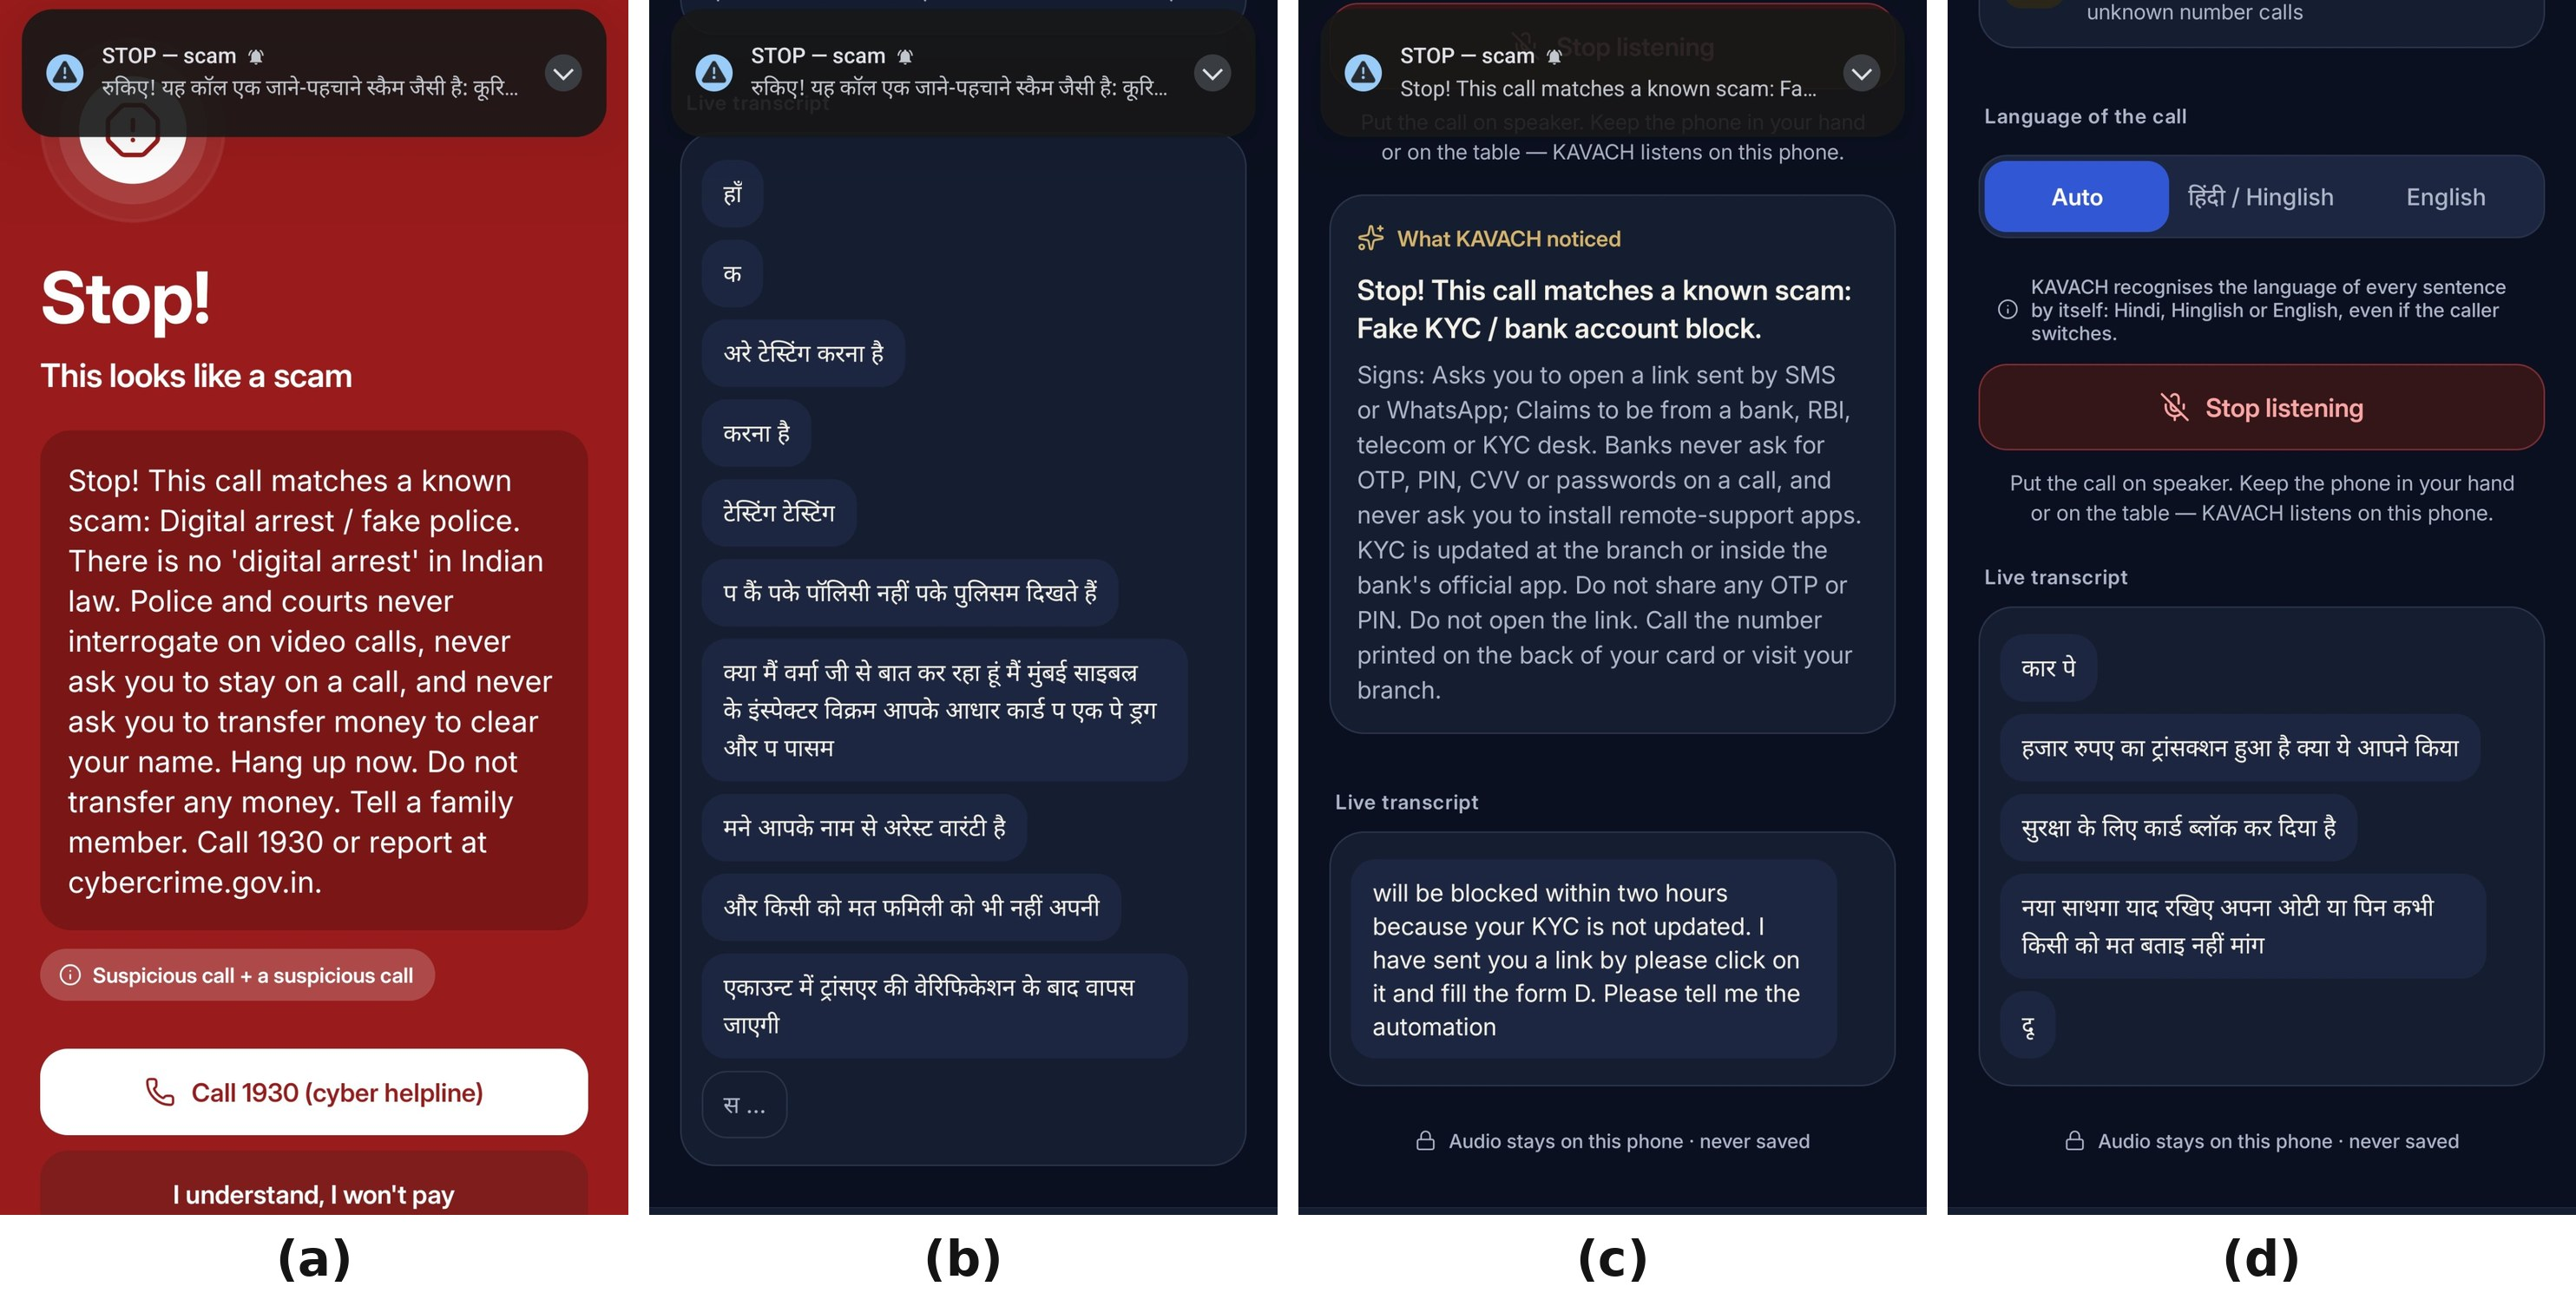
\includegraphics[width=0.92\textwidth]{fig/real_calls.jpg}
\caption{Real cellular calls from an unknown number, one phone, call on speaker, language on Auto. (a)~Hindi digital-arrest scam: full-screen Stop card during the call. (b)~Its live transcript through the phone line. (c)~English KYC scam: STOP, ``Fake KYC / bank account block''. (d)~Genuine Hindi bank fraud-check call: no warning.}
\label{fig:calls}
\end{figure*}

\subsection{Setup}
Host experiments use the sets of Table~\ref{tab:data}; thresholds were tuned on development sets only, and the hand-written and locked held-out sets were never used for tuning (the held-out set has been scored on several builds). All host results were re-run on 12 Nov 2026 with the shipped models. Audio experiments speak the calls with Piper TTS through a simulated 300--3,400\,Hz telephone band, room reverberation and noise. Phone experiments use a Xiaomi 2312DRA50I (Snapdragon~7s~Gen~2: 4$\times$Cortex-A78 at 2.4\,GHz + 4$\times$Cortex-A55 at 1.96\,GHz, 7.3\,GB RAM, Android~15), on battery. \emph{STOP before money} is the share of scam calls that reach STOP before the first payment request.

\subsection{Text classifiers}
Table~\ref{tab:text} shows the classifiers on held-out test splits. Precision is high for all three, which matters because a false alarm on a genuine message teaches the user to ignore KAVACH. Link Check flags 98.5\,\% of generated Indian look-alike domains and 0\,\% of genuine Indian domains.

\begin{table}[t]
\caption{Text classifiers on held-out test splits}
\label{tab:text}
\centering
\footnotesize
\setlength{\tabcolsep}{3pt}
\begin{tabular}{@{}lrcccc@{}}
\toprule
Model & $n$ & P & R & F1 & AUC \\
\midrule
Call window (120 tokens) & 9,010 & 0.946 & 0.883 & 0.913 & 0.962 \\
SMS / notification & 1,914 & 0.994 & 0.901 & 0.945 & 0.990 \\
URL (rules + model) & 10,196 & 0.987 & 0.752 & 0.853 & 0.945 \\
\bottomrule
\end{tabular}
\end{table}

\subsection{Call-level detection}\label{sec:calllevel}
Table~\ref{tab:guardian} replays whole calls in call time, comparing the rules alone with the shipped detector. The shipped detector raises STOP recall by 10--30 points on every set without a single false STOP (0/489, 0/498, 0/14, 0/10; with only 24 human-written genuine calls, the 95\,\% Wilson upper bound is about 14\,\%, so a $\leq$2\,\% rate is not established); its veto removed both rule-only false STOPs on the hand-written set (people \emph{discussing} a scam, and an office call about screen sharing and payments). The median time-to-STOP is under 30\,s on every set. The target of 90\,\% STOP before money is not met (50--82\,\%), and false CAUTIONs on the small hand-written and held-out sets remain high. Llama can only escalate CAUTION to STOP, so it cannot reduce false CAUTIONs. Earlier builds scored 90.6\,\%, 71.1\,\% and 70\,\% STOP on the first, second and fourth sets; the gain comes from Hindi lexicon and classifier changes made for phone failures, not from tuning on these sets.

\begin{table*}[t]
\caption{Call-level results: rules only vs.\ shipped detector (rules + classifier + veto)}
\label{tab:guardian}
\centering
\footnotesize
\begin{tabular}{@{}llcccccc@{}}
\toprule
Set (scam / genuine) & Config & STOP & $\geq$CAUTION & STOP before & Median time & False & False \\
 & & & & money & to STOP & STOP & CAUTION \\
\midrule
\multirow{2}{*}{Synthetic test (511 / 489)} & rules & 82.8\,\% & 92.4\,\% & 65.8\,\% & 17.3 s & 0\,\% & 0\,\% \\
 & shipped & \textbf{93.4\,\%} & 99.4\,\% & 82.2\,\% & 12.6 s & \textbf{0\,\%} & 5.9\,\% \\
\multirow{2}{*}{Caller through speaker (502 / 498)} & rules & 62.2\,\% & 71.7\,\% & 43.4\,\% & 18.9 s & 0\,\% & 0\,\% \\
 & shipped & \textbf{74.7\,\%} & 92.8\,\% & 60.6\,\% & 14.6 s & \textbf{0\,\%} & 5.2\,\% \\
\multirow{2}{*}{Hand-written (16 / 14)} & rules & 75.0\,\% & 87.5\,\% & 43.8\,\% & 24.7 s & 14.3\,\% & 21.4\,\% \\
 & shipped & \textbf{93.8\,\%} & 93.8\,\% & 62.5\,\% & 19.0 s & \textbf{0\,\%} & 21.4\,\% \\
\multirow{2}{*}{Locked held-out (10 / 10)} & rules & 50\,\% & 80\,\% & 20\,\% & 21.2 s & 0\,\% & 10\,\% \\
 & shipped & \textbf{80\,\%} & 80\,\% & 50\,\% & 21.3 s & \textbf{0\,\%} & 40\,\% \\
\bottomrule
\end{tabular}
\end{table*}

\textbf{Ablations (earlier builds).} Adding cue-category features raised the call classifier's test F1 from 0.817 to 0.903, and the three victim-side categories to 0.907. The victim-side cues raised STOP on the synthetic test from 88.3\,\% to 90.6\,\% and on caller-through-speaker from 68.5\,\% to 71.1\,\%, lowered hand-written false CAUTIONs from 28.6\,\% to 21.4\,\%, and added no false STOP anywhere. Template-disjoint splitting mattered most: with a development split that shared templates with training, the call classifier looked perfect on dev (F1 0.999) but reached only 0.817 on test.

\subsection{Speech in noisy rooms}
Four scripted calls were mixed with fan or traffic hum, a television, or several people talking at 30, 15, 8 and 3\,dB (48 calls per configuration; Table~\ref{tab:noise}). A larger English model let three times more noisy scam calls reach STOP. A speech denoiser helped on steady hum but invented speech-like fragments from TV and babble (WER above 1), and hotwords added one call; both were rejected. With background voices even the larger model transcribes the wrong speaker, which motivated the on-screen placement check. One TTS realisation per condition makes these numbers a direction, not precise rates.

\begin{table}[t]
\caption{English recogniser choices in noisy rooms (host)}
\label{tab:noise}
\centering
\footnotesize
\setlength{\tabcolsep}{2.5pt}
\begin{tabular}{@{}lccc@{}}
\toprule
Config. & Scam STOP & Gen. & WER \\
 & 30/15/8/3 dB & STOP & hum/TV/babble \\
\midrule
20M model & 3/6 3/6 0/6 0/6 & 0/24 & .53/.80/.74 \\
20M + denoiser & 1/24 total & 0/24 & .48/.97/1.13 \\
20M + hotwords & 3/24 total & 0/24 & .60/.74/.75 \\
Zipformer 2023 & 6/6 6/6 4/6 2/6 & 0/24 & .20/.83/.90 \\
\bottomrule
\end{tabular}
\end{table}

\subsection{Hindi speech}\label{sec:hindi}
Hindi was initially the weak link: the small streaming model turned telephone-band speech into mostly unusable text, and lexicon and classifier fixes alone raised telephone-band yellow-or-red only from 12\,\% to 44\,\% with 0\,\% red. Fig.~\ref{fig:hindi} compares it with IndicConformer on the same 100 unseen Hindi calls (50 scam, 50 genuine). On telephone-band audio STOP rose from 0\,\% to 58\,\%. Genuine calls reached STOP 0\,\% of the time and CAUTION 6\,\% (a real traffic-police call and two genuine card-fraud checks, the closest benign twins of scams).

\begin{figure}[t]
\centering
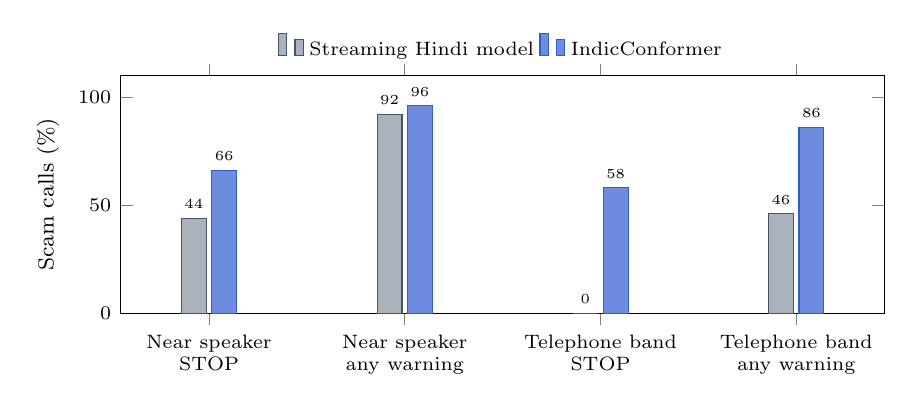
\begin{tikzpicture}
\begin{axis}[
  ybar, bar width=9pt, width=0.93\columnwidth, height=4.6cm,
  ymin=0, ylabel={Scam calls (\%)}, ylabel style={font=\footnotesize},
  symbolic x coords={Near STOP, Near any, Phone STOP, Phone any},
  xtick=data, xticklabel style={font=\scriptsize, align=center},
  xticklabels={{Near speaker\\STOP},{Near speaker\\any warning},{Telephone band\\STOP},{Telephone band\\any warning}},
  nodes near coords, nodes near coords style={font=\tiny}, ymax=110,
  legend style={font=\scriptsize, at={(0.5,1.02)}, anchor=south, draw=none, fill=none, legend columns=2},
  tick label style={font=\scriptsize}, enlarge x limits=0.15]
\addplot[fill=kgray!45, draw=kgray] coordinates {(Near STOP,44) (Near any,92) (Phone STOP,0) (Phone any,46)};
\addplot[fill=kblue!70, draw=kblue] coordinates {(Near STOP,66) (Near any,96) (Phone STOP,58) (Phone any,86)};
\legend{Streaming Hindi model, IndicConformer}
\end{axis}
\end{tikzpicture}
\caption{Hindi scam calls detected, 100 unseen calls per condition.}
\label{fig:hindi}
\end{figure}

\subsection{Auto language}
Table~\ref{tab:lang} gives LangPick's per-sentence choice on the held-out split (first two caller sentences of each call). Overall it chose the right model for 92.7\,\% of sentences (345/372). Most errors are short English sentences whose Hindi transcript is a one- or two-word fragment; the stickiness rule and the three-sentence majority limit their effect on warnings. How much a wrong choice changes the final warning is not yet measured.

\begin{table}[t]
\caption{Per-sentence language choice in Auto mode}
\label{tab:lang}
\centering
\footnotesize
\setlength{\tabcolsep}{3pt}
\begin{tabular}{@{}lcc@{}}
\toprule
Channel & English correct & Hindi correct \\
\midrule
Telephone band, 10--30 dB & 93.0\,\% (80/86) & 91.0\,\% (91/100) \\
Near speaker & 87.2\,\% (75/86) & 99.0\,\% (99/100) \\
\bottomrule
\end{tabular}
\end{table}

\subsection{Replayed and real calls on the phone}
The team's six test files played from a laptop speaker 10--30\,cm from the phone behaved as expected: Hindi digital arrest, English digital arrest and English KYC reached STOP; the English delivery and bank calls raised no warning; the Hindi genuine bank call raised only the lowest hint because of one misheard word. In an earlier build two English scams stopped at yellow because the \emph{spoken} yellow warning muted the microphone for 19--33\,s and the decisive sentences were lost; yellow warnings are now silent.

A teammate then called the test phone from a number not in its contacts over the cellular network; the call was answered in the phone's own dialer and put on speaker, and KAVACH started by itself with the language on Auto. Fig.~\ref{fig:calls} shows the results: the Hindi digital-arrest scam reached STOP during the call with a transcript close to the script; the English KYC scam reached STOP with the correct type; and a genuine Hindi bank fraud-check call (which mentions the card, a transaction, OTP and PIN) raised no warning. Three calls are a demonstration, not a statistic; the consented human-recorded set is planned next.

\subsection{Llama before and after fine-tuning}\label{sec:llamaeval}
The export pipeline was verified first: on a tiny Llama~3.2-shaped model the Hugging Face to Meta weight conversion differs by at most $3.6\times10^{-7}$ in the logits, the fp32 \texttt{.pte} with KV cache agrees step by step (max $|\Delta|$ $4.8\times10^{-7}$, 100\,\% next-token agreement), and the 8da4w \texttt{.pte} keeps 100\,\% next-token agreement.

Fig.~\ref{fig:llama} scores the base and the fine-tuned model on 100 development examples. The two failures seen on the phone before fine-tuning, advice copied from the prompt's example and English advice during a Hindi call, fell from 32\,\% to 0\,\% and rose from 55\,\% to 100\,\% correct-language respectively; quoted evidence that really appears in the transcript rose from 8\,\% to 96\,\%. These examples share the generator with the training data and use the full-precision merged model, so they measure learning of the task, not generalisation to human speech.

\begin{figure}[t]
\centering
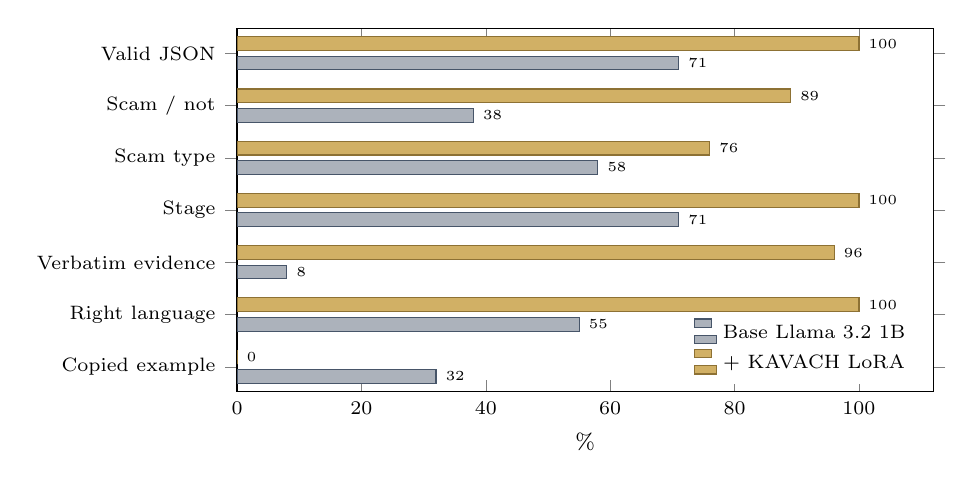
\begin{tikzpicture}
\begin{axis}[
  xbar, bar width=5pt, width=0.86\columnwidth, height=6.2cm,
  xmin=0, xmax=112, xlabel={\%}, xlabel style={font=\footnotesize},
  symbolic y coords={Copied example,Right language,Verbatim evidence,Stage,Scam type,Scam / not,Valid JSON},
  ytick=data, y tick label style={font=\scriptsize},
  nodes near coords, nodes near coords style={font=\tiny},
  legend style={font=\scriptsize, at={(0.98,0.02)}, anchor=south east, draw=none, fill=white},
  tick label style={font=\scriptsize}, enlarge y limits=0.08]
\addplot[fill=kgray!45, draw=kgray] coordinates {(71,Valid JSON) (38,Scam / not) (58,Scam type) (71,Stage) (8,Verbatim evidence) (55,Right language) (32,Copied example)};
\addplot[fill=kgold!85, draw=kgold!70!black] coordinates {(100,Valid JSON) (89,Scam / not) (76,Scam type) (100,Stage) (96,Verbatim evidence) (100,Right language) (0,Copied example)};
\legend{Base Llama 3.2 1B, + KAVACH LoRA}
\end{axis}
\end{tikzpicture}
\caption{Llama verdict quality before and after LoRA (higher is better, except ``copied example'').}
\label{fig:llama}
\end{figure}

\begin{figure}[!t]
\centering
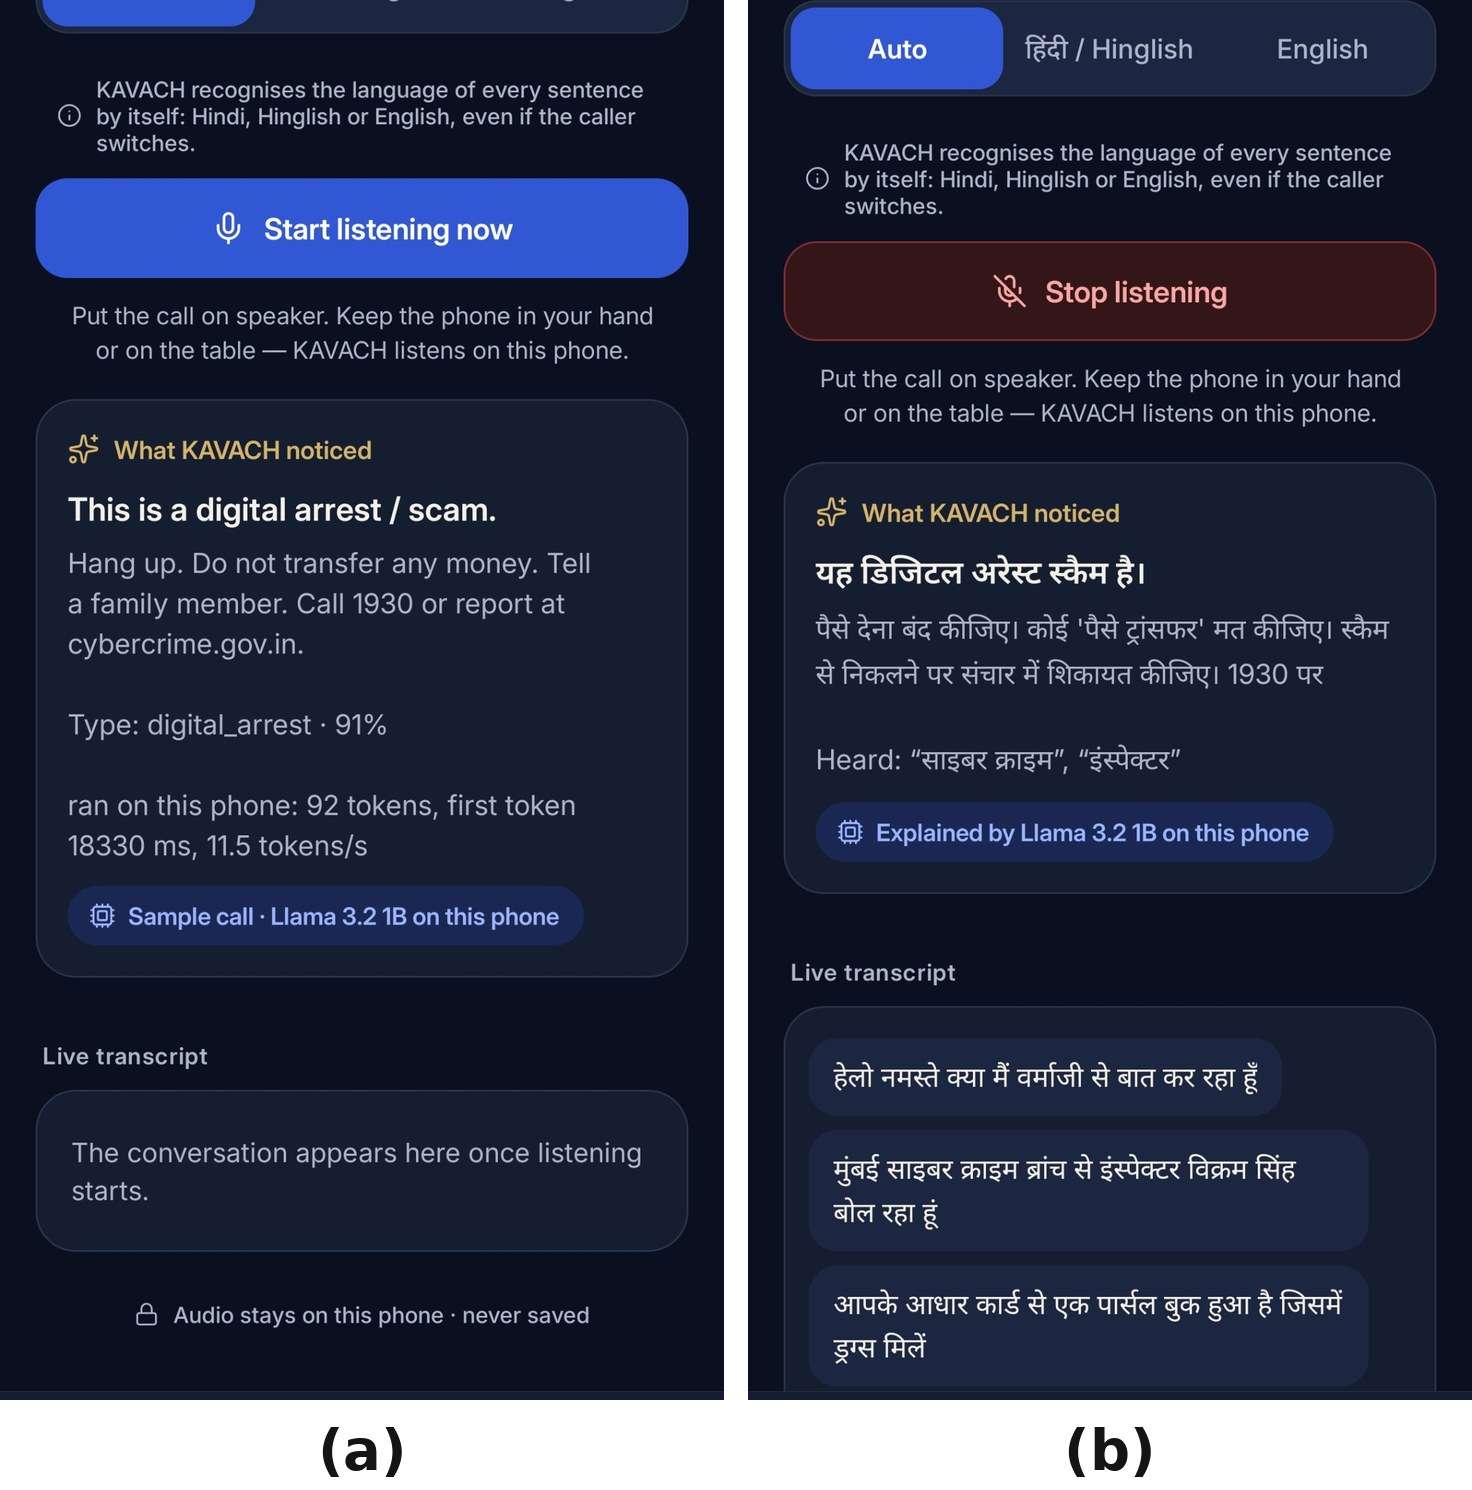
\includegraphics[width=\columnwidth]{fig/llama_phone.jpg}
\caption{Fine-tuned Llama 3.2 1B on the phone. (a)~Self-test: type \emph{digital\_arrest}, 0.91, own advice, 11.5 tokens/s. (b)~During a Hindi call: own Hindi advice with verbatim evidence, ``Explained by Llama 3.2 1B on this phone''.}
\label{fig:llamaphone}
\end{figure}

On the phone (Fig.~\ref{fig:llamaphone}) the 4-bit file loaded and ran the self-test call with verdict \emph{digital\_arrest}, confidence 0.91 and its own advice (92 tokens, 11.5 tokens/s), and during a replayed Hindi digital-arrest call it wrote its own Hindi advice with verbatim Devanagari evidence. Its Hindi is understandable but not always polished, and in one earlier run the answer was replaced by playbook text; the app now logs Llama's wording whenever that happens.

\subsection{Performance on the phone}
Table~\ref{tab:bench} lists the on-phone benchmark. Its Llama speed rows were measured with Meta's SpinQuant INT4 file before our fine-tuned file was ready; our LoRA 8da4w file decodes at 11.5 tokens/s in the on-phone self-test, so the two are on par. Real-time factor (RTF) is processing time divided by audio time. In Auto mode the two sentence models together use about $0.15{+}0.05{\approx}0.2$ of real time at two threads each, so the transcript keeps up with the caller; an hour of listening costs under 8\,\% battery with no rise in temperature. Four threads make the big models clearly faster (Hindi RTF 0.153$\to$0.092); the app uses two to save battery. Llama is the slowest component, which is why its explanation always follows the instant rule-based warning. ExecuTorch reports about 50 tokens/s for Llama~3.2~1B SpinQuant on a flagship phone, so the mid-range 11.5--11.9 tokens/s leaves room for the KleidiAI and NPU work of Phase~2.

\begin{table}[t]
\caption{Measured on the phone (Snapdragon 7s Gen 2, on battery)}
\label{tab:bench}
\centering
\footnotesize
\setlength{\tabcolsep}{3pt}
\begin{tabular}{@{}ll@{}}
\toprule
Component & Result \\
\midrule
Detector & 4.07 ms per sentence \\
IndicConformer Hindi & RTF 0.153 (2 thr), 0.092 (4 thr) \\
Parakeet 110M English & RTF 0.052 (2 thr), 0.037 (4 thr) \\
Streaming fallback (hi / en) & RTF 0.239 / 0.117 (2 thr) \\
Auto listening, 1 min & 54\,\% of one core, 385 mA (whole \\
 & phone, screen on), 235 MB, 38.0$\to$37.9\,\textdegree C \\
\multicolumn{2}{@{}l}{\emph{Llama 3.2 1B, Meta SpinQuant INT4 file (1,083 MB):}} \\
Llama load & 4.1 s, +1.1 GB \\
Llama first token & 5.9 s warm prefix, 12.9 s cold \\
Llama prefill / decode & 56--60 / 11.6--11.9 tokens/s \\
Llama while generating & 858 mA, no thermal throttling \\
\multicolumn{2}{@{}l}{\emph{KAVACH LoRA, 8da4w file (820 MB), self-test:}} \\
First token / decode & 18.3 s cold / 11.5 tokens/s \\
\bottomrule
\end{tabular}
\end{table}

\subsection{Network Watch}\label{sec:nw}
Table~\ref{tab:nw} summarises Network Watch. The rule-based traffic watch detected every simulated spyware upload, slow leak and heartbeat with no false alarms on normal apps, and the domain model caught DGA families never seen in training while flagging no genuine Indian domain. The flow model is an instructive negative result: it scores F1 0.911 on UNSW-NB15 yet flagged \emph{every} normal HTTPS session from a phone, because that data set contains no normal encrypted traffic. It therefore raises no alerts.

\begin{table}[t]
\caption{Network Watch results}
\label{tab:nw}
\centering
\footnotesize
\setlength{\tabcolsep}{3pt}
\begin{tabular}{@{}lp{0.62\columnwidth}@{}}
\toprule
Part & Result \\
\midrule
Traffic watch & 200 simulated traces per scenario: uploads, leaks, heartbeats 100\,\% detected; normal apps 0\,\% false alarms \\
Domain model & unseen DGA families: cryptolocker, necurs 92\,\%; dictionary DGAs $\approx$0\,\%; 0.36\,\% false alarms on 85k popular domains \\
Flow model & UNSW-NB15 F1 0.911; NSL-KDD~\cite{nslkdd} F1 0.854; 60/60 normal phone HTTPS flagged $\Rightarrow$ no alerts \\
Pcap demo & all 5 injected threats found, none on browsing \\
Wi-Fi check & 254 addresses in 12 s; open ADB port found \\
\bottomrule
\end{tabular}
\end{table}

\subsection{Does cross-channel fusion help?}\label{sec:fusion}
Our main novelty claim is that joining channels helps, and a rules-vs-shipped comparison does not test it. We therefore replay \emph{identical} timestamped event traces under five configurations: \textbf{A} the call detector alone; \textbf{B} message, link and app detectors alone; \textbf{C} A and B combined independently (the higher level wins); \textbf{B+} Shield with call awareness but no listening; and \textbf{D} full fusion exactly as wired in the app. Calls come from the caller-through-speaker test set, SMS texts are 8 scam and 4 genuine team-written examples, every configuration keeps the shipped thresholds, and the plan was fixed in the script before the first run (40 sessions per template; Table~\ref{tab:fusion}). D with Llama escalation is not run on the host.

\begin{table}[t]
\caption{Fusion ablation: STOPs out of 40 sessions per template (in brackets for genuine sessions: STOPs that blame the call)}
\label{tab:fusion}
\centering
\footnotesize
\setlength{\tabcolsep}{3pt}
\begin{tabular}{@{}lcccc@{}}
\toprule
Template & A & C & B+ & D \\
\midrule
\multicolumn{5}{@{}l}{\emph{Scam sessions}} \\
Scam call alone & 37 & 37 & 0 & 37 \\
+ scam SMS with link, mid-call & 32 & 40 & 40 & 40 \\
+ APK install & 30 & 30 & 40 & 40 \\
+ remote access, then payment app & 36 & 36 & 40 & 40 \\
Scam SMS 5 min before the call & 30 & 37 & 33 & 40 \\
First 40\,\% of the call, then APK & 7 & 7 & 40 & 40 \\
\midrule
\multicolumn{5}{@{}l}{\emph{Genuine sessions}} \\
Genuine call alone & 0 & 0 & 0 & 0 \\
+ unrelated scam SMS mid-call & 0 & 32 (0) & 32 (22) & 40 (32) \\
+ scam SMS 20 min after the call & 0 & 32 (0) & 32 (0) & 32 (3) \\
+ payment app during the call & 0 & 0 & 0 & 4 (4) \\
+ risky APK 2 days earlier & 0 & 0 & 0 & 0 \\
+ genuine SMS, duplicated, reordered & 0 & 0 & 0 & 0 \\
+ work screen sharing, no payment & 0 & 0 & 40 (40) & 40 (40) \\
\bottomrule
\end{tabular}
\end{table}

Fusion turns an ambiguous call into STOP \emph{at the risky action} (an install during the call: 30$\to$40; a call heard only in part: 7$\to$40), but the share of scams warned \emph{before} the risky step is identical for C and D in every template, so it does not warn earlier. Most of the gain comes from knowing that an unknown-number call is in progress (B+); what was heard adds 3/40 when a scam SMS preceded the call. The costs are concrete: an unrelated scam SMS during a genuine call is blamed on the call (32/40), and screen sharing for work during an unknown-number call is STOP by design. The rules join events by time only; matching the organisation named on the call with the sender of a message is future work.

\subsection{Targets}
Table~\ref{tab:targets} compares the Phase~1 targets with what was measured. Eight are met, one is partly met, one cannot be shown with the available genuine calls, and one is missed.

\begin{table}[t]
\caption{Targets vs.\ achieved}
\label{tab:targets}
\centering
\footnotesize
\setlength{\tabcolsep}{3pt}
\begin{tabular}{@{}llll@{}}
\toprule
Target & Goal & Achieved & Met \\
\midrule
Network use & none & no \texttt{INTERNET} & \checkmark \\
Audio stored & none & memory only & \checkmark \\
Languages & hi, en, auto & 92.7\,\% per sentence & \checkmark \\
Detector & $<$10 ms & 4.07 ms & \checkmark \\
Speech speed & $>$ real time & $\approx$5$\times$ & \checkmark \\
Median to STOP & $<$30 s & 12.6--21.3 s & \checkmark \\
False STOP & $\leq$2\,\% & 0 observed & not shown \\
STOP before money & $\geq$90\,\% & 50--82\,\% & -- \\
LLM on Arm CPU & 1B, 4-bit & 11.5--11.9 tok/s & \checkmark \\
Battery & $<$10\,\%/h & $\approx$7.6\,\%/h (1 min) & partly \\
Real calls & correct & 3/3 & \checkmark \\
\bottomrule
\end{tabular}
\end{table}

\section{Discussion and Limitations}\label{sec:disc}

\textbf{Lessons.} Five findings changed the design. (1)~Speech quality, not the detector, limited Hindi: no lexicon fix recovered telephone-band Hindi until the recogniser changed. (2)~Speaking a warning during a call mutes the listener, so in-call warnings must be silent. (3)~Android can silently revoke a running accessibility service, so the app must verify capture rather than trust a settings switch. (4)~Benchmark-trained network models can fail completely on phone traffic, so a model with a good F1 still has to be tested on the target device's data. (5)~Joining channels by time alone helps at the risky action but can blame an innocent call (Section~\ref{sec:fusion}).

\textbf{Evasion.} Table~\ref{tab:evasion} lists the main ways a scammer may try to avoid KAVACH and the defence for each.

\begin{table}[t]
\caption{Evasion attempts and defences}
\label{tab:evasion}
\centering
\footnotesize
\setlength{\tabcolsep}{3pt}
\begin{tabular}{@{}p{0.36\columnwidth}p{0.56\columnwidth}@{}}
\toprule
Evasion & Defence \\
\midrule
Avoid trigger words & classifier and category combinations; Llama reads meaning \\
Clean talk, send link / APK & unknown call + risky action is STOP \\
Calm with small talk & level sticky within a session \\
Switch language & per-sentence Auto choice \\
Spoken prompt injection & Llama cannot lower STOP; verbatim evidence only \\
\bottomrule
\end{tabular}
\end{table}

\textbf{Limitations.} All accuracy numbers except the three real calls use synthetic text or TTS voices from one voice per language; human voices, accents and crowded rooms will score lower. The always-on detector misses 7--25\,\% of scam calls depending on the set, and the ``warned before payment'' rate (50--82\,\%) is below our 90\,\% target. The battery figure extrapolates a one-minute, whole-phone sample; a sustained soak with an idle baseline is pending. The deployed 4-bit Llama is only observed on the phone, its confidence is self-reported and uncalibrated, and prompt-injection resistance rests on the output contract rather than a measured attack rate. Llama's Hindi is understandable but not always polished. Listening requires the call on speaker and the accessibility permission running; a store version would need a phone maker's system mode or a declared accessibility use case. Network Watch rules are evaluated on simulated traces.

\textbf{Ethics.} KAVACH listens only to unknown-number calls the user has chosen to protect and stores no audio; the main app cannot use the network, and the optional family SMS, paired Bluetooth link and DNS-watch app are off unless the user enables them. Role-play recordings are collected only with written consent, and no real victim data is used. Zero false STOPs is a hard target because a false STOP on a genuine bank call could stop a user from acting on a real fraud alert.

\section{Conclusion and Future Work}\label{sec:concl}
KAVACH shows that a mid-range Arm phone can hear, understand and explain a scam call in Hindi or English while the call is happening, entirely offline: two speech models and a millisecond detector together used about half of one CPU core in a one-minute run, a 1B-parameter LLM explains alerts at 11.5--11.9 tokens/s, no genuine call was stopped in any evaluated set, and three real calls were handled correctly. Phase~2 will (i)~record 100+ scam and 100+ genuine consented role-play calls as an untouched human test set and adapt the recognisers; (ii)~score the deployed 4-bit Llama on independent, ASR and prompt-injection prompts and measure how much it raises STOP before payment; add entity-aware fusion; (iii)~run the quantisation ladder with KleidiAI on and off, on big and LITTLE cores and on a budget phone, with a 30-minute soak and an idle baseline; (iv)~move the speech encoders to the NPU and compare energy with the CPU; and (v)~run a consent-based pilot with 20--30 family volunteers.

\section*{Acknowledgment}
The authors thank Dr. Rahul Ratnakumar for his guidance, the organisers of the Arm Bharat AI-SoC Challenge 2026--27, and the open-source projects this work builds on: Meta Llama, ExecuTorch, AI4Bharat IndicConformer, NVIDIA Parakeet, sherpa-onnx, Silero VAD, Piper and wordfreq.

\begin{thebibliography}{99}
\bibitem{mha_loss} Scroll, ``Indians lost Rs 22,845 crore to cyber fraud in 2024, a 206\% rise from previous year: Centre,'' Jul. 2025. [Online]. Available: \url{https://scroll.in/latest/1084796/indians-lost-rs-22845-crore-to-cyber-fraud-in-2024-a-206-rise-from-previous-year-centre}
\bibitem{mha_da} Inc42, ``Indians lost INR 1,935 Cr to digital arrest scams in 2024: Govt,'' Mar. 2025. [Online]. Available: \url{https://inc42.com/buzz/indians-lost-inr-1935-cr-to-digital-arrest-scams-in-2024-govt}
\bibitem{conformer} A. Gulati \emph{et al.}, ``Conformer: Convolution-augmented transformer for speech recognition,'' in \emph{Proc. Interspeech}, 2020, pp. 5036--5040.
\bibitem{fastconformer} D. Rekesh \emph{et al.}, ``Fast Conformer with linearly scalable attention for efficient speech recognition,'' in \emph{Proc. IEEE Autom. Speech Recognit. Underst. Workshop (ASRU)}, 2023.
\bibitem{ctc} A. Graves, S. Fern\'andez, F. Gomez, and J. Schmidhuber, ``Connectionist temporal classification: Labelling unsegmented sequence data with recurrent neural networks,'' in \emph{Proc. Int. Conf. Mach. Learn. (ICML)}, 2006, pp. 369--376.
\bibitem{indicvoices} T. Javed \emph{et al.}, ``IndicVoices: Towards building an inclusive multilingual speech dataset for Indian languages,'' in \emph{Findings Assoc. Comput. Linguist. (ACL)}, 2024.
\bibitem{parakeet} NVIDIA, ``parakeet-tdt\_ctc-110m,'' model card, 2025. [Online]. Available: \url{https://huggingface.co/nvidia/parakeet-tdt_ctc-110m}
\bibitem{sherpa} k2-fsa, ``sherpa-onnx: speech recognition, synthesis and VAD with ONNX Runtime,'' 2025. [Online]. Available: \url{https://github.com/k2-fsa/sherpa-onnx}
\bibitem{silero} Silero Team, ``Silero VAD: pre-trained enterprise-grade voice activity detector,'' 2024. [Online]. Available: \url{https://github.com/snakers4/silero-vad}
\bibitem{llama3} A. Grattafiori \emph{et al.}, ``The Llama 3 herd of models,'' \emph{arXiv preprint arXiv:2407.21783}, 2024.
\bibitem{spinquant} Z. Liu \emph{et al.}, ``SpinQuant: LLM quantization with learned rotations,'' \emph{arXiv preprint arXiv:2405.16406}, 2024.
\bibitem{executorch} PyTorch Team, ``ExecuTorch: On-device AI inference for PyTorch,'' 2025. [Online]. Available: \url{https://github.com/pytorch/executorch}
\bibitem{kleidiai} Arm Ltd., ``KleidiAI: micro-kernels for AI workloads on Arm CPUs,'' 2025. [Online]. Available: \url{https://gitlab.arm.com/kleidi/kleidiai}
\bibitem{lora} E. J. Hu \emph{et al.}, ``LoRA: Low-rank adaptation of large language models,'' in \emph{Proc. Int. Conf. Learn. Represent. (ICLR)}, 2022.
\bibitem{hashing} K. Weinberger, A. Dasgupta, J. Langford, A. Smola, and J. Attenberg, ``Feature hashing for large scale multitask learning,'' in \emph{Proc. Int. Conf. Mach. Learn. (ICML)}, 2009, pp. 1113--1120.
\bibitem{killchain} E. M. Hutchins, M. J. Cloppert, and R. M. Amin, ``Intelligence-driven computer network defense informed by analysis of adversary campaigns and intrusion kill chains,'' Lockheed Martin Corp., Tech. Rep., 2011.
\bibitem{androidaudio} Android Developers, ``Share audio input,'' 2025. [Online]. Available: \url{https://developer.android.com/media/platform/sharing-audio-input}
\bibitem{wordfreq} R. Speer, ``wordfreq: Access a database of word frequencies in many languages,'' 2022. [Online]. Available: \url{https://github.com/rspeer/wordfreq}
\bibitem{rbi_bankin} Reserve Bank of India, circular RBI/2025-26/28 on the exclusive ``.bank.in'' domain for banks, 2025.
\bibitem{unsw} N. Moustafa and J. Slay, ``UNSW-NB15: a comprehensive data set for network intrusion detection systems,'' in \emph{Proc. Military Commun. Inf. Syst. Conf. (MilCIS)}, 2015.
\bibitem{piper} Rhasspy, ``Piper: a fast, local neural text to speech system,'' 2024. [Online]. Available: \url{https://github.com/rhasspy/piper}
\bibitem{smsspam} T. A. Almeida, J. M. G. Hidalgo, and A. Yamakami, ``Contributions to the study of SMS spam filtering: New collection and results,'' in \emph{Proc. ACM DocEng}, 2011.
\bibitem{nslkdd} M. Tavallaee, E. Bagheri, W. Lu, and A. A. Ghorbani, ``A detailed analysis of the KDD CUP 99 data set,'' in \emph{Proc. IEEE CISDA}, 2009.
\end{thebibliography}

\end{document}
